\documentclass[10pt,a4paper,danish]{article}
%% Indlæs ofte brugte pakker
\usepackage{amssymb}
\usepackage[danish]{babel}
\usepackage[utf8]{inputenc}
\usepackage{listings}
\usepackage{fancyhdr}
\usepackage{hyperref}
\usepackage{booktabs}
\usepackage{graphicx}
\usepackage{algorithmic}
\pagestyle{fancy}
\fancyhead{}
\fancyfoot{}
\rhead{\today}
\rfoot{\thepage}

% Opsæt indlæsning af filer
\lstset{
  language=Python,
  extendedchars=\true,
  inputencoding=utf8,
  linewidth=\textwidth, basicstyle=\small,
  numbers=left, numberstyle=\footnotesize,
  tabsize=2, showstringspaces=false,
  breaklines=true, breakatwhitespace=false,
}

%% Titel og forfatter
\title{Informationsteknologi: Projekt e-læring \\ Projektkursus: Systemudvikling \\Forår 2011}
\author{Arinbjørn Brandsson (hkt789)\\Lasse Ahlbech Madsen (xsc606)\\Naja Mottelson (vsj465)\\Søren Pilgård (vpb984)\\
\\
Gruppeid : LO6\\
\\Instruktor: Lasse Nørregaard}

%% Start dokumentet
\begin{document}

%% Vis titel
\maketitle
\newpage

%% Vis indholdsfortegnelse
\tableofcontents
\newpage

%% HER STARTER RAPPORTEN
\section{Formål}
\subsection{Systemdefinition}
Systemet består af et digitalt interaktivt læringsværktøj hvis mål er at indføre elever på gymnasiefaget Informationsteknologi i programmering af systemer i forskellig størrelse. Disse systemer vil primært være fokuseret på udvikling af spil, men bredt datalogisk kompetencegivende. Systemet opbygges som et hjælpeprogram, som kører ved siden af brugerens teksteditor og en række præetablerede programmeringsforløb som eleven kan deltage i. Et forløb består af en række trin - konkrete programmeringsopgaver som hver indeholder en beskrivelse, en række hints samt et sæt tests der holder styr på om brugeren har opfyldt målet for hvert trin. Når brugeren har gennemgået alle trinene vil vedkommende have et komplet spil der kan afvikles seperat fra udviklingsværktøjet. Systemet vil blive udviklet som en skrivebordsapplikation der kan afvikles lokalt på den enkelte brugers datamat/foldedatamat eller på datamater i gymnasiets eventuelle it-rum.

\subsection{BATOFF}
\begin{itemize}
\item \textbf{Betingelser}: Gymnasieelever med begrænsede programmering- og systemudviklingserfaringer. 
\item \textbf{Anvendelsesområde}: Eleven som bruger af systemet. Hvis værktøjet instaleres centralt på et
gymnasiums datamater vil der typisk være en Itadministrator hvis rolle er at opsætte systemet.
\item \textbf{Teknologi}: Systemet designes til at kunne køre på almindelige hjemmedatamater/foldedatamater.
Systemet vil blive baseret på python samt forskellige biblioteker dertil (i særdeleshed biblioteket pygame)
\item \textbf{Objekter}: En bruger som udvikler et spil i forbindelse med et forløb af opgaver. 
\item \textbf{Funktion}: Udvikling af spil.
\item \textbf{Filosofi}:  Digitalt interaktivt læringsværktøj
\end{itemize}

\section{Kravsspecifikation}
Den kravsspecifikation vi har arbejdet med bygger på følgende krav:

\begin{enumerate}
\item Systemet skal kunne oprette nye forløb, samt tilgå gamle, ikke-gennemførte forløb lagret lokalt på brugerens datamat. 
\item Systemet skal indeholde funktioner til at registrere om et forløb er gennemført af en bruger. 
\item Systemet skal indeholde flere forskellige læringsforløb som brugeren kan gå i gang med.  
\item Systemet skal ikke tilbyde en integreret teksteditor.
\item Systemet skal indeholde funktionalitet til at køre brugerens kode samt fremvise fejlbeskeder.
\item Systemet skal for hvert (relevant) trin i en programmeringsopgave tilbyde en tekst med hints og links til relevant dokumentation.
\item Brugergrænsefladen skal ligne (om end ikke være 100 procent ens med) figurerne (henvisning til figurerne)
\item Systemet skal være intuitivt at arbejde med - kun det programmeringsfaglige skal være krævende. 
\item Systemet skal kunne køre på både Windows, Mac og Linux
\item Systemet skal ikke stille hardware-krav som ikke mødes af størstedelen af almindelige hjemme-PC'er.
\end{enumerate}  

Vi har i arbejdet med projektet lagt vægt på følgende designkriterier (opdelt efter vigtighed og
hvorvidt det er opnået): 
\begin{table}[h!]
  \begin{center}
    \begin{tabular}{llllll}
      \toprule
      Kriterium & Meget   & Vigtigt & Mindre  & Irrelevant & Trivielt \\
                & vigtigt &         & vigtigt &            & opfyldt  \\
      \midrule
      Brugbart        & &x& & & \\
      Sikkert         & & & &x& \\
      Effektivt       & & &x& & \\
      Korrekt         & & &x& & \\
      Pålideligt      & & &x& & \\
      Vedligeholdbart & & &x& & \\
      Testbart        & & & &x& \\
      Fleksibelt      &x& & & & \\
      Forståeligt     & &x& & & \\
      Genbrugeligt    & & &x& & \\
      Flytbarhed      & &x& & & \\
      Integrerbart    &x& & & & \\
      \bottomrule
    \end{tabular}
    \caption{Kvalitetsattributter for klienten.}
    \label{tab:kvalitetsattributter_program}
  \end{center}
\end{table}

\section{Den tekniske platform}
Teknisk består vores program af 4 lag (startende nederst): python, pygame-biblioteket, 
spilskelettet og vores applikation sammen med brugerens editor. \\

Her vil python vil være den bærende del (da selve applikationen er kodet i dette sprog), 
og pygame-bibliioteket bruger vi til at håndtere ting som 2d grafik, lyd og tastaturinput. 
Spilskelettet er den ufærdige kildekode til spillet som brugeren får udleveret og skal bygge
videre på.
\\
Øverst har vi et todelt lag bestående af vores applikation samt brugerens editor.
Det vil være gennem dette lag at brugeren inteagerer med de dybere lag.

\section{Arkitektur}

\subsection{Komponentarkitektur}
Vores komponentarkitektur er opdelt i tre lag: klienten 
(hvis ansvar det er at hente dataet fra de forskellige trin og vise dem), modelkomponentet
(som opbevarer de forskellige trin og holder styr på hvor langt brugeren er i forløbet
og således hvilke trin der kan blive vist og hvilke hints der kan blive givet)
og så de tests der bliver kørt i forbindelse med hvert trin. To komponenter kan 
siges at agere sideløbende med vores program, navnligt brugerens eget tekstredigeringsværktøj
og selve det spil som brugeren arbejder på, som lagres lokalt på brugerens datamat. 

\subsection{Procesarkitektur:} Vores system bliver udført på gymnasiets datamater eller
elevernes egne foldedatamater. Potentielle 
problemer med samtidige processer forventes at blive løst af operativsystemet. 
Kontrollen over vores system ligger i modelkompnentet  og klientkomponentet, hvilket er 
håndteret af operativsystemet (og i mindre grad, af den tekst editor som brugeren 
bruger). 

\subsection{Standarder:} Designet af de forskellige vinduer og fejlbeskeder vil følge ikke følge 
en bestemt standard, da vi vil integrere dem med vores system så at de passer med 
vores systems design. 

\section{Modelkomponent og Funktionskomponent}
\subsection{Modelkomponentet}
Vores modelkomponenet holder styr på hvor langt brugeren er i forløbet og
hvilke tests, der skal køres på dennes kode. Desuden holder det styr på, hvor
mange hints, der er vist.

\subsubsection{Klasser i modelkomponentet}
Klassen "Bruger" er hvor det bestemmes hvilken opgaver man har og ikke har
lavet, hvor klassen "Opgaver" bestemmer de forløb en bruger kan være i gang med
eller have gennemørt. Under klassen "Spil" valgte 
vi at generalisere de to states "Færdig" og "Ikke Færdig/Fejl", hvilket bestemmer om brugeren 
har lov til at fortsætte med den næste opgave, eller skal arbejde videre med den 
opgave som de er i gang med. Klassen "Test" refererer til de grupper af tests
der er associeret med hvert enkelt trin, og som modellen kalder når klienten 
signalerer at brugeren er nået til et bestemt trin.  

\subsection{Funktionskomponent}
Vi har som sådan ikke rigtig arbejdet med et separat funktionskomponent, eftersom vores
modelkomponent indeholder de funktioner som kontrollerer programmet (i 
samarbejde med klienten). Man kan muligvis argumentere for at klienten selv 
er en form for funktionskomponent, da det er denne del af programmet der 
signalerer til modelkomponentet hvor brugeren er i et forløb - dog er 
klienten også ansvarlig for opgaven at vise selve grænsefladen for brugeren, og
kan ikke kaldes udelukkende et funktionskomponent. 

\section{Brugergrænsefladekomponent}
Som det også forklares i afsnittet om projektarbejdet: Siden Delrapport 3 har vores 
indsats udelukkende været fokuseret omkring udvikling af de forskellige trin der udgør
det første forløb (fem af disse er vedlagt som bilag til denne rapport). Vi har derfor
på nuværende tidspunkt ingen kodet brugergrænseflade at fremvise. 

\paragraph{}
Vores tanker vedr. struktureringen af brugergrænsefladekomponentet er at det vigtigste
er at græsefladen er så enkel som muligt, for ikke at forvirre brugeren unødigt. Dette
er heldigvis en overkommelig opgave da grænsefladen hovedsageligt vil skulle fremvise
trin, som udelukkende består af nemt overskuelig tekst. 

\paragraph{}
Vores plan er at dele græsefladen op i 3 overorndede vinduer:

\paragraph{}
Det første vindue (kaldet startup) vil stille brugeren overfor valget enten at starte et 
nyt forløb eller fortsætte på et der allerede er etableret.
Hvis brugeren vælger at fortsætte på et tidligere startet forløb, vil en dialogboks komme 
frem hvori han kan navigere hen til forløbet og fortsætte på det.
Hvis brugeren derimod vælger at starte et nyt forløb bliver han dirregeret til hovedevindue
nummer 2. Vinduet består af 3 knapper for at holde tingene så simple som muligt: 
\begin{itemize}
\item \textit{Start nyt forløb} knappen
\item \textit{Fortsæt tidlligere forløb} knappen
\item \textit{Hjælp} knappen der åbner en dialogboks hvor man kan læse om brugen af programmet.
\end{itemize}

\paragraph{}
Det andet vindue (kaldet initialisation) vil være der hvor brugern kan starte et nyt forløb og
indtaste navn og sti i filsystemet (hvor forløbet skal gemmes).
Det er også her hvor brugern skal finde ud af hvilket forløb han vil gå igang med: De forskellige
forløb vil præsentere hvilket spil de laver, hvad man lærer af at lave dette spil samt hvor svært/hvilke
 krav der til brugeren før han kan gå igang (f.eks. at brugeren har styr på de grundlæggende dele af python)
Når brugeren er klar kan han trykke start.

\paragraph{}
Det tredje vindue er selve applikationen.
Vinduet er tænkt at fylde i højden men ikke i bredden.
Her vil man have en række knapper til at navigere med, samt et større område med tekst.
Øverst vil der sidde 4 knapper: 
\begin{itemize}
  \item En tilbage knap, symboliseret med en pil der peger mod venstre.
  \item En kør knap der starter spillet.
  \item En hjælp knap med et spørgsmålstegn der åbner hjælpesiden som i vindue 1.
  \item En frem knap symboliseret med en pil mod højre.
\end{itemize}

\paragraph{}
For at opnå en forståelse af hvordan vi har tænkt os at brugergrænsefladen 
kommer til at tage sig ud, har vi vedlagt figurene \ref{fig:startvindue}, 
\ref{fig:hovedvindue} og  \ref{fig:nytforloeb} som viser vores tegnede mockups
af grænsefladen. \begin{figure}[h]
  \begin{center}
    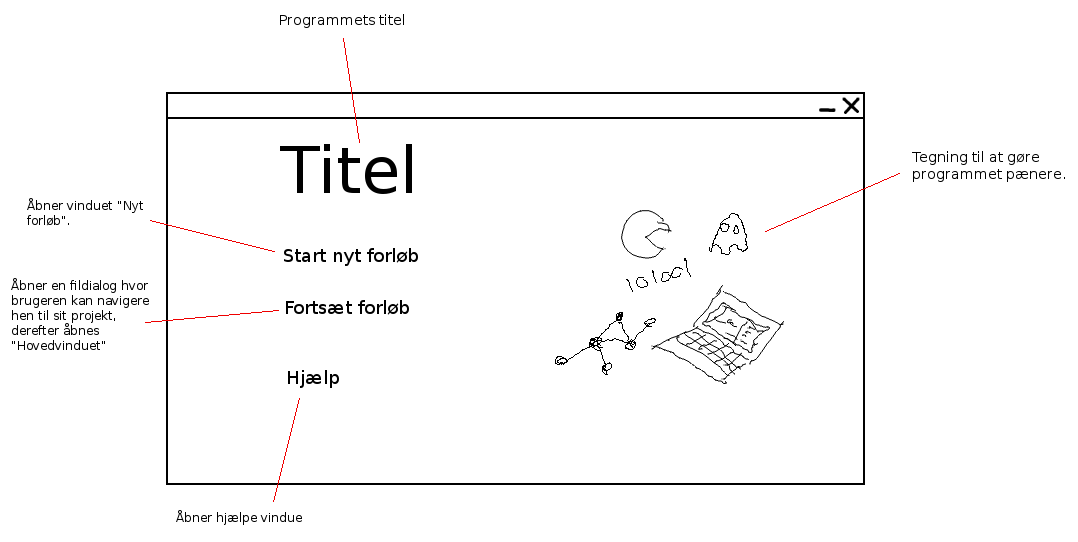
\includegraphics[scale=0.4]{startvindue.png}
    \caption{Programmets startvindue}
    \label{fig:startvindue}
  \end{center}
\end{figure}
\newpage

\begin{figure}[h]
  \begin{center}
    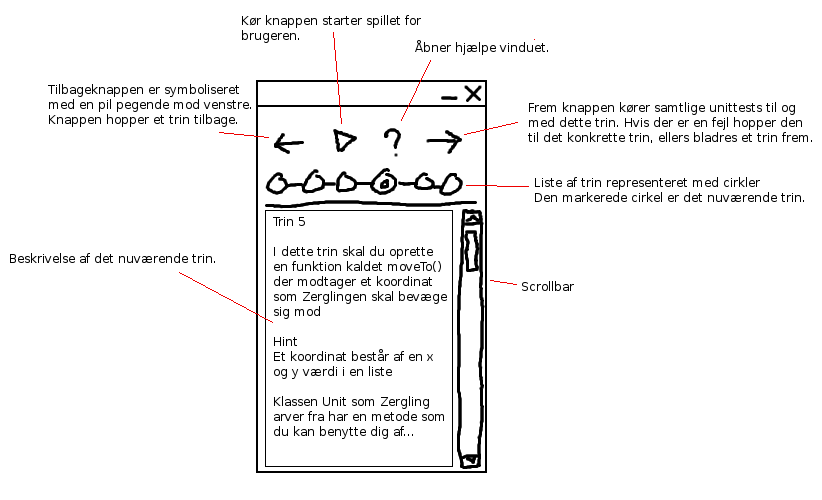
\includegraphics[scale=0.4]{hovedvindue.png}
    \caption{Programmets hovedvindue}
    \label{fig:hovedvindue}
  \end{center}
\end{figure}
\newpage

\begin{figure}[h]
  \begin{center}
    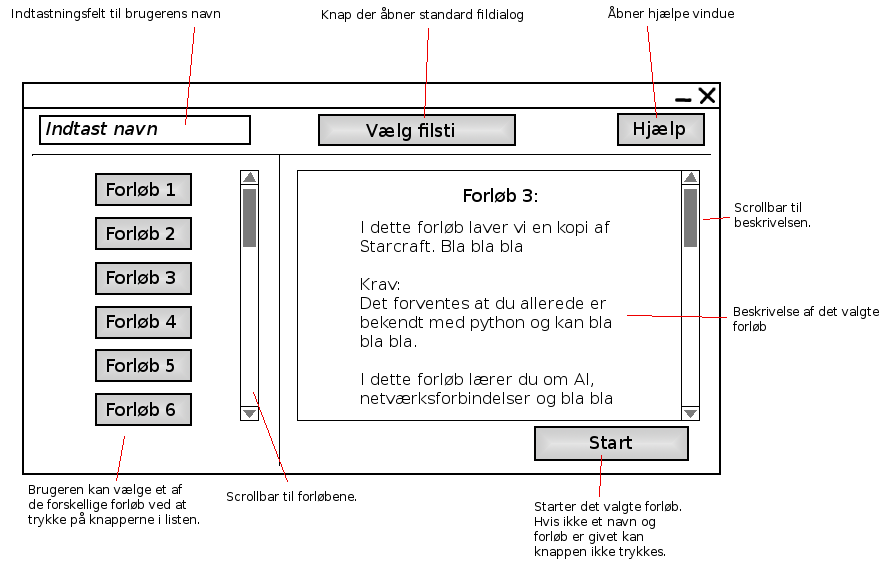
\includegraphics[scale=0.4]{nytforloeb.png}
    \caption{Et nyt forløb}
    \label{fig:nytforloeb}
  \end{center}
\end{figure}
\newpage

\section{Implementering af IT-løsningen}
Status på implementeringen af selve klienten (som er det egentlige produkt 
i dette projekt) er desværre på samme status som brugergrænsefladen. Hvad vi
har fokuseret på at kode hidtil har været det spil der fungerer som det 
underliggende data for klienten, og som de enkelte trin tager udgangspunkt i.

\paragraph {} 
Hele spillet er på nuværende tidspunkt kørende og afprøvet, og indeholder al den data vi
gerne ville have at give brugere i udviklingsarbejdet (bl.a. har vi lavet
en række ikoner til brug i tegningen af de forskellige entititeter i spillet). 
Den kildekode der er vedhæftet denne rapport er fra spillets model.py-modul, som
lagrer alle klasserne i spillet samt enkelte af de metoder de deler. 

\paragraph {} 
Alt i alt består vores spil af følgende moduler: 
\begin{itemize}
\item \textit{game.py} indeholder \"main\" metoden, det er herfra spillet startes. Derudover indeholder den selve spilløkken.
\item \textit{model.py} indeholder alle de klasser der er i spillet, her er alle spilobjekterne defineret.
\item \textit{data.py} er en slags database over alt i spillet. Modulet holder styr på de forskellige spilkonstanter så som vinduestørrelsen, samt sæt af spillets objekter. Når et nyt objekt bliver oprettet skal det tilføje sig i de relevante grupper så de bliver opdateret og vist korrekt.
\item \textit{mapping.py} banerne til spillet består af simple tekstfiler der indlæses og gemmes i data modulet. Når banerne er blevet indlæst er der funktionalitet i mapping modulet der kan omsætte banen til faktiske objekter.
\item \textit{direction.py} Udgør enums for alle 4 verdenshjørner, modulet bliver brugt til bevægelse af spilleren.
\item \textit{functions.py} indeholder enkelte funktioner som var for generelle til at passe ind i andre moduler.
\item \textit{resources.py} indeholder alt funktionalitet der har med faktisk indlæsning af data at gøre.
\end{itemize}

Udover disse filer findes to mapper \textit{images} som indeholder alt billedmaterialle, samt \textit{maps} der indeholder banefiler.

\section{Projektsamarbejdet}
\subsection{Projektstyring}
Siden sidste rapport har langt størstedelen af vores arbejde været rettet imod
fremstilling af trinene til projektet og klargøring af test af disse. Fem af trinene
er vedlagt nærværende rapport (se bilag). Processen
omkring begge disse opgaver har været langt fra optimal: Selve udfærdigelsen af 
trinene trak ud længere end det burde have gjort, eftersom samtlige gruppemedlemmer
har været under forskellige former for tidspres, og generelt været dårlige til 
at delegere tilstrækkelig tid til projektet. Selve afprøvningen er blevet presset
af at vores kundes elever gik på læseferie inden vi kunne igangsætte afprøvningen. 

Vi udviklede trinene ved først at uddelegere 2-3 trin til hvert enkelt gruppe-
medlem, og derefter satte vi os sammen og strømlinede dem, så de blev ens i
format og tilgang. Dette viste sig at være en rigtig god måde at tvinge alle
til at være kreative, og komme med deres bud på en løsning. På nuværende tidspunkt
er 10 ud af 13 trin i det første forløb blevet færdigproducerede. Dette er ikke 
optimalt, men tilstrækkeligt til at kunne udføre sigende tests.

I Delrapport 3 fremsatte vi hensigten at uddele selve projektopgaven i 4 hovedområder
(projektstyring, kode, afprøvning, dokumentation) og uddelegerede ansvar for hvert 
område til et enkelt gruppemedlem. Siden da har det vist sig at denne idé måske var
for ambitiøs: Vi har slet ikke haft tid eller overskud til at arbejde på alle områder, 
og sidste ende ikke været nogen grund til at holde hinanden i tovene på de forskellige
områder. I stedet har vi kørt med den samme model som hidtil, hvor vi har en person med 
det overordnede ansvar. Det er stadig ikke optimalt, og vi har stadig problemet at det 
ikke er alle gruppemedlemmer som har fuldt overblik over projektet.
Det skaber meget mere arbejde for dem der rent faktisk har det,
og sætter de resterende medlemmer værre i en eksamenssituation.

\subsection{Møder med brugeren}
Siden delrapport 3 har vi afholdt ét yderligere møde med kunden, i form af 
den afprøvningssession der beskrives i afsnit 8. Alt i alt vil dette sige 
at vi har afholdt 3 møder med vores kunde (udover vores korrespondance pr. 
mail og telefon) - et indledende møde hvor vi mødte eleverne og blev enige
med deres underviser om projektets udformning, et møde hvor vi afprøvede 
papir-mockups og afslutningsvis det møde der beskrives nedenfor. 

\subsection{Referat- og dokumentationsstrategi}
Alt i alt har vores referater under projektets forløb været forholdsvis 
kaotiske. I projektets begyndelse har vi ført meget grundige (og hyppige)
referater, som på nuværende tidspunkt ikke fremstår så nyttige eftersom 
en stor del af selve projektet har ændret sig drastisk siden da. 

Det har vist sig at sidste rapports ide med at fordele hovedansvaret for
forskellige dele af projektet var lidt for ambitiøs. Vi har slet ikke haft tid
eller overskud til at arbejde på alle delene, og i sidste ende har der slet
ikke været nogen grund til at holde hinanden i tovene på de forskellige områder.
I stedet har vi kørt med den samme model som hidtil, hvor vi har en person med
det overordnede ansvar. Det er stadig ikke optimalt, og vi har reelt kun den ene
person med et egentlig overblik over projektet. Det skaber mere arbejde for den
ansvarlige,og sætter de 3 andre medlemmer værre i en eksamenssituation, når de
skal redegøre for forløbet og de forskellige projektdele.

I de møder vi har haft, har vi nok engang haft sløsede referater, men de har
heller ikke været så relevant, da alt vores arbejde og tanker røg ned på papir
i forbindelse med de trin vi har udviklet. Vi har
siden sidste rapport ikke oplevet problemer med opmøde, ud over at folk stadig
kommer for sent. Ideen med at lægge møderne i forlængelse med undervisningen
var som sådan ikke en dårlig ide, men det er som regel mest praktisk at lægge
møderne tidligere på dagen, og folk har det tilsyneladende bedre med at komme
for sent til disse end undervisning. 

Vores valg af versionsstyringsværktøj fungerer til gengæld glimrende. Vi har nu alt vores
arbejde delt og sorteret i mapper og alt er let tilgængeligt. Folk har en meget
god forståelse for hvordan GitHub fungerer, og der er på nuværende tidspunkt ikke
nogen der oplever problemer med at bruge det. Den eneste problematik vi oplever 
på dén front er at nogle gruppemedlemmer ikke altid pusher så snart de er færdige 
med en opgave, hvilket gør det besværligt at danne sig et overblik over hvor langt 
vi er med enkelte delopgaver uden at skrive ud på mailinglisten eller at pinge folk
provat. Dette er meget frustrerende, i sær eftersom det er et problem der er blevet
påpeget og kritiseret gentagne gange i løbet af projektet. 

\subsection{Perspektivering}
\subsubsection{Projektstyring generelt}
En overordnet ting vi alle sammen har oplevet i dette projekt er at vores valg
af generel ansvarsfordeling ikke har fungeret. Modellen hvor et enkelt menneske
har ansvar for selve projektstyringen fungerer sandsynligvis udmærket i professionel
sammenhæng og på større projekter, men i vores størrelsesorden og niveau har det
simpelthen ikke fungeret. Når man arbejder sammen så få mennesker, og i så løbende 
kontakt som man gør som studerende, gør det næsten mere skade end gavn at have et 
enkelt menneske med mere ansvar end resten af gruppen. Da vi traf beslutningen om 
at organisere os på denne måde var vi i en lidt anden situation, med et yderligere 
medlem i gruppen. Havde vedkommende ikke faldet fra projektet kunne vi muligvis
have haft nytte af denne måde at organisere os på, men det kan jo ikke blive andet
end spekulation på nuværende tidspunkt. 

Vi har gennem forløbet arbejdet en del med at forbedre vores dokumentations-
strategi, til tider fungerede den godt, med aktions-reaktions skemaer for vores
interviews, men til vores møder formåede vi aldrig at få skabt en god standard.
De fleste af vores referater kan ikke bruges til meget mere end at tjekke
egentlige beslutninger. I et fremtidigt projekt ville vi absolut udbedre dette,
og bl.a. få argumenter og begrundelser med for de valg vi traf, så vi i mod-
sætning til nu, kan se hvorfor vi valgte at gøre som gjorde.

Vi valgte i processen at bruge en betragtelig mængde energi på det pædagogiske indhold
af vores projekt, og på at finde ud af hvad selve spillet skulle gå ud på o. lign. På 
denne måde er vores implementationsarbejder blevet meget forhalet, resulterende i at
vi ikke kommer til at have en kørende prototype på det planlagte tidspunkt. I retrospekt
ville en god idé have været at påbegynde implementeringen sideløbende (eller, potentielt, 
inden) analysearbedet, så at vi ville have en base af fungerende programmel at udvide
på i takt med at projektets indhold blev mere veldefineret.

I et fremtidigt projekt vil vi endvidere forsøge at være hårdere med deadlines da dette har
været et gennemgående problem i gruppen, og har skabt stress og dårligere
produkter. Det er dog svært at rette på, når det er et generelt problem i
gruppen, og vi ikke har adgang til andre konsekvenser end at forlade gruppen.
Det bliver uundgåeligt noget med at forsøge at holde hinanden i ørerne, og
forsøge at holde konstant opsyn med status på forskellige opgaver, hvilket er
generende for alle i gruppen. 

Alt i alt er det der generer os mest, at vi har set os nød til at fokusere mere
på at skrive rapporter, end at udvikle et produkt vi kunne være tilfreds med.
Her et par uger før eksamen står vi ikke med noget der ligner et færdigt program,
og det er ikke, fordi det er et voldsomt stort eller kompliceret program, men
fordi rapporterne syntes at fylde mere end udviklingen. 

\subsubsection{Valg af kunde og kundekontakt}
Vi kunne godt have brugt mere kontakt med kunden, eftersom vi syntes at det blev meget "vores" projekt
i stedet for et vi lavede i fællesskab. Specielt i starten virkede det heller ikke som om, at vi 
havde den samme forståelse af meningen med projektet, og det ønskede produkt.
Dette kunne bestemt gøres bedre, og ville forventeligt være anderledes i en
situation, hvor vi var hyret til en opgave, i stedet for at vi er ude og sælge
et projekt, som vi godt kunne tænke os at lave. Hvis der var en kontrakt invol-
veret, ville det nok også have været anderledes, da kunden ville være mere 
opsøgende i forhold til status og den videre udvikling af projektet, i stedet
for passivt at vente på, hvad vi nu finder på at aflevere. Det var en risiko vi
tog, da vi valgte at arbejde sammen med en enkelt gymnasielærer i de stressede
månederne op til gymnasieeksamenerne. Dette skulle vi måske have været mere
bevidste om. 

Ved indgangen til projektet stod vi overfor to alternativer til den kunde vi endte med
at vælge at samarbejde med. En anden samarbejdspartner vi kunne have valgt at arbejde med
var foreningen DKUUG, som var meget interesseret i et projekt af lignende tilskæring, om end
med andet fagligt fokus end spiludvikling. Endvidere havde vi, udover tilbuddet fra Greve
Gymnasium, muligheden for at samarbejde med et yderligere gymnasium og på denne måde fordoble
mængden af gymnasieelever at bruge som testpersoner. 

Vi har generelt haft besvær med at komme ordentligt i kontakt med vores kunde på Greve Gymnasium. 
Dette kan der have været mange forskellige grunde til - bl.a. kom vi jo ind i deres undervisningscyklus
på et meget sent tidspunkt, hvilket måske bidrog til at dæmpe både underviserens og elevernes 
interesse i at deltage i projektet. I sær her til sidst har vi haft meget svært ved at få fat
på gymnasiet, af den simple grund at studentereksaminerne er gået i gang og både lærerens og
elevernes prioriteter nu (forståeligt nok) ligger et helt andet sted. Vi forestiller os at vi ville
have haft præcis de samme problemer hvis vi havde valgt et andet gymnasium at samarbejde med, samt 
hvis vi havde valgt at arbejde med to sideløbende. Faktisk ville samarbejde med to gymnasier potentielt
have været ret skadeligt for projektet, da det ville fordoble den (i forvejen betragtelige) opgave 
at holde kontakt til kunden, informere om fremskridt og deltage i løbende møder. 

I retrospekt ville et samarbejde (enten eksklusivt eller som én kunde sideløbende med et gymnasium) med 
DKUUG måske have været en god idé. Et problem vi oplevede løbende med Greve Gymnasium var at gymnasielæreren
vi havde størstedelen af vores kontakt med lod til at opfatte det som 'vores' projekt i højere grad end 
hans som kunde. Han havde derfor ofte ikke så meget at bidrage med, hvilket gjorde at vi var nødt til at
bestemme størsteden af kravene til systemet samt det pædagogiske indhold selv. Dette har vi ikke været tilfredse
med, fordi det i høj grad har tilføjet til vores arbejdsbyrde i projektet. Folk fra DKUUG ville potentielt
havde kunnet fratage os en del af dette ansvar, af den simple grund at de ville have bedre idé om præcis
hvilken slags program de kunne tænke sig at ende op med. 

\subsubsection{Analysearbejdet}
En mere overordnet (og egentlig mere problematisk) observation vi har gjort os er at det projekt vi 
har valgt ikke passer særlig godt på den analysemetode vi benytter på kurset. Selvom spillet selv 
er objektorienteret er den applikation som er det egentlige program ret svært at beskrive med de 
væktøjer og modeller der stilles til rådighed i bogen. Dette har betydet at en del af de opgaver der
har været i forbindelse med forfatning af delrapporter har fungeret som yderligere arbejdsopgaver
snarere end at hjælpe os med at udvikle og forstå programmet vi har arbejdet på. Når vi næste gang
påbegynder et projekt vil vi derfor gøres os umage med at vælge projekt og analysemetode der rent 
faktisk understøtter hinanden på en produktiv måde. 

\section{Afprøvning med brugerne}
Som nævnt i delrapport tre har vores afprøvning med brugerne (i dette tilfælde gymnasieelever)
været en del anderledes end afprøvning beskrevet i kursuslitteraturen af den grund at vi ikke 
har en kørende prototype af selve klienten til vores program. Hvad vi valgte at gøre var 
derfor i stedet at fokusere på at afprøve det pædagogiske indhold i de trin vi har udfærdiget
til programmets første udviklingsforløb. Dette involverede dog også en del forberedelse, i 
særdeleshed i forbindelse med at udvælge det materiale der skulle afprøves. 

Som nævnt i forgående afsnit havde vi indledningsvist meget svært ved at få kontakt til de 
testpersoner vi gerne ville benytte i Greves datalogiklasse. Vi endte dog med at aftale en 
afprøvningssession på to timer med tre elever d. 31. maj. Heraf dukkede to af dem op. Dette viste sig dog
at fungere meget godt, da vi hurtigt løb tør for tid og det potentielt ville have krævet flere resourcer
at have flere testpersoner.

\subsection{Overvejelser og forberedelse inden afprøvningen}
En stor del af de trin vi har udarbejdet indeholder python- eller pygamespecifik information (se vedlagte bilag), som 
vi gerne ville undgå at forudsætte for meget af. Vi valgte derfor at fokusere på de helt 
grundlæggende funktionaliteter i spiludviklingen, som nemmest kunne abstraheres og gøres forståelige.
Et kriterium for de ting vi stillede spørgsmål til var at de såvidt muligt var nemme at
forestille sig uden at tænke for meget på specifikke implementeringsdetaljer (fx. ville vi gerne undgå
ting som input handling, som kræver et vist kendskab til håndtering af tastaturinput, og ting som 
fokuserede for meget på matematiske udregninger, da mange har svært ved at udføre den slags på stående fod). 
Vi valgte derfor at fokusere på at stille spørgsmål til opbygningen af de forskellige entitetsklasser i spillet
(spilleren selv, vægge, monstre, guld), udvalgte dele af klassernes opførsel i spillet (hovedsageligt collision
detection), samt den grundlæggende funktionalitet i main-funktionen. 

Ca. en uge inden mødet havde vi sendt dem en mail med en kort introduktion til hvordan afprøvningen 
ville foregå, samt links til information som de med fordel kunne sætte sig ind i inden afprøvningen 
(grundlæggende objektorientering, pygame). Med i denne mail var desuden en kort beskrivelse af det spil
vi ville stille dem spørgsmål til. 

\subsection{Afprøvningen}
Afprøvningen foregik ved at vi indledningsvist gentog de grundlæggende rammer for det
spil vi ville arbejde med (hvad en spiller skulle kunne, 
hvordan reglerne ifbm. monstre og guld var). Herefter foregik afprøvningen af de
udvalgte trin ved at vi læste højt/forklarede den beskrivelse der indleder hvert 
trin, og stillede de spørgsmål som trinnet indeholdt. I tilfælde hvor trinnene
fokuserede på teknisk specifikke ting (fx. pygames klasser eller datastrukturer) 
valgte vi at omformulere spørgsmålene så at de blev mere generelle. I tilfælde hvor 
opgaverne i trinnene afhang af kendskab til data eller funktionalitet i andre dele 
af programmet valgte vi enten at skitsere kort hvad der var i bemeldte del af programmet, 
eller omformulere opgaven så at den blev uafhængig af den programdel. Når testpersonerne havde
svært ved at forstå opgaven eller ikke kunne komme på en måde at løse opgaven
gav vi dem de hints der ligeledes indgår i hvert trin. 

Selve afprøvningen uspillede sig ikke 100 procent optimalt. Ved begyndelsen sagde
begge testpersoner at de ikke havde haft tid til at sætte sig 
ind i python (dette havde vi heller ikke som sådan forudsat), pygame eller havde nogen 
erfaring med spiludvikling overhovedet. Dette viste sig at blive problematisk, fordi 
vi gentagne gange blev nødt til at forklare dem hvordan overordnede ting i spiludviklingen
fungerer, såsom nedarvning og konstruktion af klasser og tilhørende metoder. Disse forklaringer
var i høj grad af information som var at finde i de links der blev henvist til i trinnene, 
men det optog en del tid og vi havde indtryk af at testpersonerne havde svært ved at 
håndtere så store mængder information på én gang. 

Spørgsmålene til de allerførste trin foreløb forholdsvis kaotisk. Selve main-loopet
blev vi nødt til at forklare i ganske høj detaljeringsgrad for at vores testpersoner
kunne forstå det, og selv herefter blev vi hurtigt nødt til at fokusere på modellen
i spillet fordi selve main-funktionen var svær for dem at forestille sig. Spørgsmålene
til de enkelte klasser forløb en del bedre: Begge elever var i stand til at komme med 
bud på hvilke metoder de forskellige klasser skulle indeholde, og efter noget tid (og
yderligere forklaring) kunne den ene af testpersonerne give et bud på hvordan Player-klassen
kunne initialiseres, samt hvordan man kunne lave funktionalitet til at få spilleren 
til at samle guld op og blive angrebet af et monster. Hans bud på hvordan man kunne gøre 
det var anderledes end den måde vi selv har implementeret det, men i testens kontekst
var det så meget som vi håbede på.

Som afprøvningen skred frem blev vi ret hurtigt nødt til at stille spørgsmål til 
opgaver der lå udenfor de trin vi havde planlagt at spørge til. Dette var af den 
simple grund at vi forholdvis hurtigt løb tør for spørgsmål som eleverne kunne løse
på stående fod, og var nødt til at prøve at finde på andre ting at spørge om. I særdeleshed
havde begge elever svært ved at forstå spørgsmålene til collision detection og 
hvordan/hvor de klasser de havde beskrevet skulle initialiseres og sættes i brug. Vi 
forsøgte os med at stille spørgsmål til de udvidede metoder til de forskellige klasser
(move og update) men selv efter gentagne forklaringer og hints kunne
ingen af eleverne give bud på hvordan nogen af metoderne kunne implementeres. 

Begge elever sagde at en stor del af deres besvær med at løse de opgaver
vi stillede dem havde at gøre med at de ikke følte sig sikre nok til at kunne
komme med bud på algoritmer uden at kunne sidde og lege med det på egen hånd.
De mente begge to at de ville kunne løse (de nemmere af) opgaverne alene, hvis
de havde den fornødne tid til at læse de links der indgik i trinene og kunne
sætte sig mere ind i python, pygame og objektorientering generelt. 


\subsection{Overvejelser efter afprøvningen}
Alt i alt synes vi at vores afprøvningssession med de to elever blev ret kaotisk.
Af de specifikke ting de to elever havde svært ved er det svært at skelne imellem
hvad der har at gøre med det faglige niveau i opgaverne og hvad der har at gøre med
vores testpersoners manglende forberedelse og forvirring over den uvante måde at 
skulle løse datalogiske problemer. Det lader dog til at de opgaver der har at gøre
med de mere matematiske/abstrakte dele af programmet (fx. collision detection og move-metoden)
skal forklares meget mere grundigt, og måske deles op på flere forskellige trin for
at uvante programmører kan følge med. Det samme kan siges om de trin der har at gøre 
med selve main-loopet. En måde at løse problematikken ved main-funtkionen og main-loopet
ville være at give brugeren mere funktionalitet i skelettet der udleveres, så at 
de kan se hvordan det bliver gjort i stedet for at skulle lave så meget af det
fra bunden. 

Begge elever virkede dog positivt stemte overfor idéen om programmet som helhed, 
og syntes at (de mindre krævende af) opgaverne var sjove. Begge af dem var af den 
mening at de, hvis de havde bedre tid og måske fik mere udførlige beskrivelser i de 
svære trin, ville kunne gennemføre forløbet i sidste ende. 

\section{Diskussion af artikel}
Artiklen "Designing the Handheld Maritime Communicator" handler om processen som omfattede at
lave et system som ville være ansvarlig for at sørge for sikkerheden når risikabelt arbejde skulle udføres 
i store fragtskibe. Artiklen går i dybde med dette, hvor den beskriver alle trinene bag systemet, fra 
udformningen af systemet, til interviews med klientellet, indsamlingen af det information som skulle 
bruges, designet af systemet, og til sidst den måde som designerne af systemet besluttede at teste systemet, 
(både brugertests og bugtesting). Fremgangsmåden som programmørerne brugte til at designe systemet vil blive 
analyseret samt sammenlignet med kursuslitteraturen.

I stedet for interviews med deres klientel tog nogle medlemmer af holdet med på nogle af skibene for længere perioder, 
(Det siges ikke hvor længe), hvor de tog noter om hvordan opgaver var klaret, (som for eksempel hvis sømændene skulle 
få deres last om bord på skibet). Ud over dette tog de også noter om problemer med den måde som sømændene klarede 
disse problemer på, som så skulle løses. Holdet tog også lyd-og-video analyser, hvor de tog lyd segmenter eller 
video segmenter fra om bord på et skib, og kiggede dem igennem. Dette var gjort så at holdet kunne få en bedre 
idé om forholdene på skibene, samt også for at se hvilken ordrer der blev typisk givet. Deres plan var at bruge disse 
til at kunne lave forprogrammerede kommandoer. Denne måde som holdet brugte til at få information vedrørende det 
det system som deres kunde havde brug for er meget anderledes end den metode som Back to Thinking Mode havde 
argumenteret for, hvor man skulle have adskillige interviews med sin kunde, hvor man skulle føre en dagbog. Her brugte 
man hovedsageligt et 'action-reaction' type format. Dog kan man argumentere at denne fremgangsmåde 
ville ikke virke for dette projekt, da holdet havde brug for at have en klar idé om hvad arbejderne havde brug for, og 
ikke hvad deres chefer havde brug for, samt hvis de havde foretaget interviews i stedet for feltarbejde ville holdet ikke 
få at vide hvilken kommandoer var typisk givet fra kaptajnen eller lignende højrestående arbejdere.

Mens systemet stadig var i koncept-fasen lavede holdet et klassediagram og et papir mockup om systemet for at vise 
hvordan systemet skulle virke. Klassediagrammer er et udbredt fænomen i større projekter, som er beskrevet i bogen 
"Objekt Orienteret Analyse og Design", som er brugt til at give et samlet overblik over problemområdet, hvilket 
er nyttigt for dette system da systemet skulle kunne holde styr på skibbet, opgaverne og det team som skulle 
udføre disse opgaver. Klassediagrammer er effektive da de hjælper med at holde et overblik over systemet, og 
også til at hjælpe folk med at se hvilken klasser har hvilken effekt på hvilken klasser. Papir mockups, som også 
er diskuteret i "Cardboard Computers: Mockingit-up or Hands-on the Future", hjælper med at få folk til at forstå 
hvilken grænseflader holdet syntes vil være den bedste IT-løsning. Dette er en effektiv måde at vise et holds kunder 
hvilken grænseflader de syntes vil være effektive, da de er hurtigere at lave i forhold til at lave prototyper, hvilket 
betyder at et hold kan eksperimentere med forskellige design. Og da dette systems design er altafgørende, (da systemet 
skulle være nemt og hurtigt at bruge for arbejderne), var det en umådelig god idé at lave forskellige papir mockups i stedet 
for at lave mange forskellige prototyper.

Holdet som designede systemet brugte et såkaldt 'iterativ design'. Iterativ design fungerer ved at holdet 
laver en prototype. Denne prototype bliver så testet, analyseret og refineret, hvorefter holdet kigger 
på hvad der skal laves om eller skal ændres. Disse ændringer bliver inkluderet i en ny prototype, som gennemgår 
de samme trin som før indtil man har et færdigt produkt. Denne form for design er meget anderledes end et 
traditionelt vandfaldsmodel, (hvor man antager at hvert trin bliver udført perfekt, og skal ikke ændres), eller et 
spiralmodel, (fra "A Spiral Model of Software Development and Enhancement"), hvor man lavede en prototype  
for hver gang man havde startet et nyt trin. Selvom et iterativ design er mere tidskrævende en et 
vandfaldsmodel eller et spiralmodel, vil et iterativ design sørge for at når systemet bliver udleveret 
vil der være færre bugs, problemer og ueffektive designelementer. Dette er meget vigtigt for et sikkerhedssystem, 
da det kan koste liv hvis der sker en fejl. Artiklen "Designing for Usability: Key Principles and What The Designers 
Think" er enig med at et iterativt design er den mest effektive designproces, da et iterativt designproces vil eventuelt 
finde mange, hvis ikke alle, designproblemer, som for eksempel tvetydige beskeder. Artiklen give endda et eksempel 
på et problem som et hold havde, hvor brugerne misforstod nogle af de kommandoer som de kunne bruge, som iterativt design 
rettede op på. Tvetydige kommandoer eller funktioner ville have været et stort problem for projektet for brugerne, så 
det var en god idé at bruge et iterativt designproces til systemet.

\section{Bilag}
\section{Trin}
\subsection{Trin 2: Oprettelse af Player-klassen}
\subsubsection{Skelet:}
\begin{verbatim}
Class player(pygame.sprite.Sprite):
    def __init__(self, x, y):
\end{verbatim}
\subsubsection{Beskrivelse:}
Du skal nu oprette en af de mest grundlæggende ting i spillet: selve spilleren.
Vi gør dette ved at oprette en klasse (Player) som nedarver fra en klasse der
er indbygget i pygame (Sprite). Det er hvad du kan se i det indbyggede skelet. 
Eftersom din Player arver alle de metoder som Sprite-klassen har, bliver en 
god del af din opgave at finde ud af hvilke metoder og attributter du vil bruge.
Som det første skal du sørge for at din Player får indhentet et ikon, så den kan 
blive tegnet på en bane (yderligere funktionalitet følger senere). 
\\
\subsubsection{Hints:}
\begin{enumerate}
\item Kig i resources.py. Er der funktionalitet der gør noget af 
det du har brug for der? Hvad returnerer de funktioner der er defineret
i det modul?
\item Overvej hvilke attributter en spiller egentlig har brug for, udover
et billede. Hvor er han henne? Hvor er han på vej hen? 
\item Overvej om du kan kombinere indhentningen af billedet med indhentning
af anden information om spilleren.
\item Kig grundigt på dokumentationen til pygames Sprite-klasse. Er
der noget du kan bruge? 
\end{enumerate}

\subsubsection{Links:}
\begin{enumerate}
\item Pygames dokumentation til Sprite-klassen: http://www.pygame.org/docs/ref/sprite.html
\item Introduktion til Sprite-klassen: http://www.pygame.org/docs/tut/SpriteIntro.html
\item Generel spil-tutorial som (bl.a.) benytter Sprite--klassen: http://pygame.org/docs/tut/chimp/ChimpLineByLine.html
\end{enumerate}

\subsection{Trin 7: Oprettelse af Wall-klassen}
\subsubsection{Skelet:} 
\begin{verbatim}
class Wall(pygame.sprite.Sprite):
    def __init__(self, x, y):
\end{verbatim}

\subsubsection{Beskrivelse:}
Nu hvor du har en bane og en spiller der kan rykke
rundt på den er det på tide at lave nogle mure som 
kan gøre banen lidt mere spændende. Som enhver trænet
koder tænker du øjeblikkeligt på at oprette en klasse
til at modellere vægge. 
\\
En væg deler visse karakteristika med en spiller:
De kan begge nedarve fra pygames Sprite-klasse, og 
alle væggens grundlæggende metoder vil også kunne
findes hos spilleren. 
\\
Når du har oprettet væg-klassen skal du sørge
for at væggene bliver lagret det rigtige sted
i spillet. 

\subsubsection{Hints:}
\begin{enumerate} 
\item Prøv at overvej hvad en mur egentlig består af,
   samt hvad den skal kunne. Skal den kunne flytte sig?
   Skal den have et billede? Hvordan spiller disse 
   to ting sammen?
\item Hvor ligger informationerne om de ting der er 
   at finde på en bane? Hvordan sørger du for at
   væggen bliver placeret dér når dens init-metode
   bliver kaldt?
\end{enumerate}

\subsection{Trin 8: Collision detection }
\subsubsection{Skelet:} 
\begin{verbatim}
Intet skelet udleveres til dette trin. 
\end{verbatim}
\subsubsection{Beskrivelse:}
Du skal nu tilføje 'collision detection'. Dette skal bruges
til at sørge for at din spiller f.eks. ikke kan stå oven i 
mure. Dette skal implementeres som en del af move-metoden i 
player klassen, som du oprettede tidligere.
Collision detection kan man med fordel kode med udgangspunkt
i de biblioteker du får fra pygame.

\begin{enumerate}
\item Et godt udgangspunkt er metoden spriteCollide fra den gammelkendte
Sprite-klasse. 
\item Når du specifikt skal undgå at din spiller går ind i mure, hvilke 
argumenter skal din metode så bruge?
\item Hvordan sørger du for at der ikke er mere én sprite på en bestemt
position?
\end{enumerate}

\subsubsection{Links:}
\begin{enumerate}
\item Wikipedias artikel om collision detection: http://en.wikipedia.org/wiki/Collision\_detection
\item Tutorial om collision detection i pygame: http://www.switchonthecode.com/tutorials/collision-detection-with-pygame
\item Grundlæggende pygame-tutorial indeholdende helt basal introduktion til collision detection
og rects: http://pygame.org/docs/tut/newbieguide.html
\item Endnu en tutorial (også indeholdende sprite-grupper): http://www.devshed.com/c/a/Python/PyGame-for-Game-Development-Sprite-Groups-and-Collision-Detection/
\end{enumerate}

\subsection{Trin 6: Input handling}
\subsubsection{Skelet:} 
\begin{verbatim}
def handle_input():
    for event in pygame.event.get():
            if event.key == pygame.K_UP:
                ''Få spilleren til at skifte retning''
            elif event.key == pygame.K_DOWN:
                ''Få spilleren til at skifte til en anden retning''
\end{verbatim}
\subsubsection{Beskrivelse:}
Du skal nu kode den del af spillet der håndterer input fra spilleren - 
dvs. at du skal få spillet til at reagere på det data det modtager fra
tastaturen (fx. når spilleren trykker på piletasterne). I handle\_input() 
skal du konkret finde ud af at stoppe spillet, samt at få spilleren til 
at bevæge sig vha. input fra tastaturet. 
//
Måden vi gør dette i pygame er vha. såkaldt hændelseshåndtering (event
handling). Dette står beskrevet i nærmere detaljer under links-sektionen. 
//
Som du kan se af kodeskelettet lægger vi ud med at indhente en liste 
(også kaldet en kø) af hændelser fra tastaturet (ln 1). Denne undersøger 
vi herefter, og angiver hvordan spillet skal reagere på beskeder fra de 
forskellige taster (eksempel: ln 2-5). 

\subsubsection{Hints:}
\begin{enumerate}
\item Størstedelen af det data der skal manipuleres her er spillerens retning.
   Hvor lagres det?

\item Hvilket tastaturinput virker bedst til at bestemme retning på spilleren?
   Hvornår vil du indhente dataet fra tasterne - når de er blevet trykket ned
   eller når de er blevet sluppet igen?

\item Du skal (ud fra en hændelse fra tastaturet) få spillet til at stoppe. Hvor
   har du en funktion der stopper spillet?

\item Du kan hente inputtet til at stoppe spillet på flere måder - bl.a. har 
   pygame en indbygget quit-konstant. Hvordan kan du ellers stoppe spillet?
   Er der behov for flere måder at stoppe spillet på?

\item Undersøg forskellen på de to hændelsestyper pygame.KEYUP og pygame.KEYDOWN. 
   Skal spillet reagere forskelligt på de to?
\end{enumerate}
\subsubsection{Links:}
\begin{enumerate}
\item Pygames hændelseshåndteringsmodul: http://www.pygame.org/docs/ref/event.html
\item Pygames liste af tastatur-konstanter: http://www.pygame.org/docs/ref/key.html
\item Kort opsummering af begerebet hændelseshåndtering: http://en.wikipedia.org/wiki/Event\_handler
\item Mini-tutorial om hændelseshåndtering: http://lorenzod8n.wordpress.com/2007/05/30/pygame-tutorial-3-mouse-events/
\item Pygames egen tutorial om hændelser mm. : http://inventwithpython.com/chapter18.html
\end{enumerate}

\subsection{Trin 10: Oprettelse af Gold-klassen}
\subsubsection{Skelet:} 
\begin{verbatim}
Intet skelet udleveres. 
\end{verbatim}
\subsubsection{Beskrivelse:}
Nu hvor vi har en spiller og en bane med mure kan du 
oprette præmier som din spiller kan samle op. Som det 
både var tilfældet med spilleren og væggene skal du
oprette en klasse til at modellere dine præmier. 
//
Udover de standardattributter som klassen skal have
(billede, rect etc), bør du overveje hvordan denne 
klasse skal relatere sig til Player-klassen. Hvad skal 
der ske når spilleren samler en præmie op? Hvilken 
klasse skal opdateres i det tilfælde?
//
Når du har oprettet klassen skal du (selvfølgelig)
sørge for at den bliver tiløjet til data.py det
rigtige sted. Du skal dog også kigge på hvor du
kan initialisere dine præmier, så at de bliver
tegnet i den bane der bliver spillet på.  

\subsubsection{Hints:}
\begin{enumerate}
\item Overvej helt præcis hvad der skal ske
når din spiller samler en præmie op. Har du
brug for en metode til at simulere det?
\item Er der andre klasser der skal opdateres
nu hvor du har en præmie-klasse?
\item Overvej hvilken del af programmet der 
lagrer information om hvad der er til stede 
på selve banen. Hvordan kan du sørge for at
dine præmier bliver initialiseret dér?
\end{enumerate}
\subsubsection{Links:}
\begin{enumerate}
\item Der er ingen links til dette trin. 
\end{enumerate}

\section{Kildekode}
\lstinputlisting{model.py}

\end{document}
